\documentclass[12pt]{article}
\usepackage{tikz}
\usetikzlibrary{positioning,shapes}

\begin{document}

\begin{center}
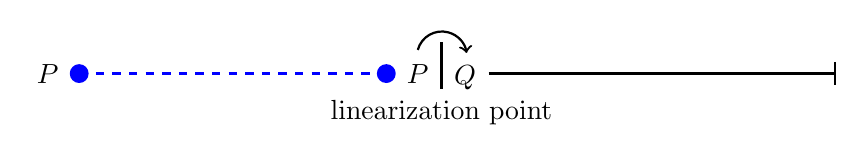
\begin{tikzpicture}[thick]
\node (Ps) at (0, 0) {$P$};
\node (P) at (4.7, 0) {$P$};
\node (Q) at (5.3, -0.05) {$Q$};
\node (L) at (5, -0.5) {linearization point};

\filldraw[color=blue] (0.4, 0) circle (3pt);
\filldraw[color=blue] (4.3, 0) circle (3pt);
\draw[color=blue, dashed] (0.4, 0) -- (4.3, 0);
\draw (5, 0.4) -- (5, -0.2);
\draw (5.6, 0) -- (10, 0);
\draw (10, 0.15) -- (10, -0.15);
\draw [->] (4.7, 0.3) arc (165:8:9pt); 
\end{tikzpicture}
\end{center}

\iffalse
\begin{center}
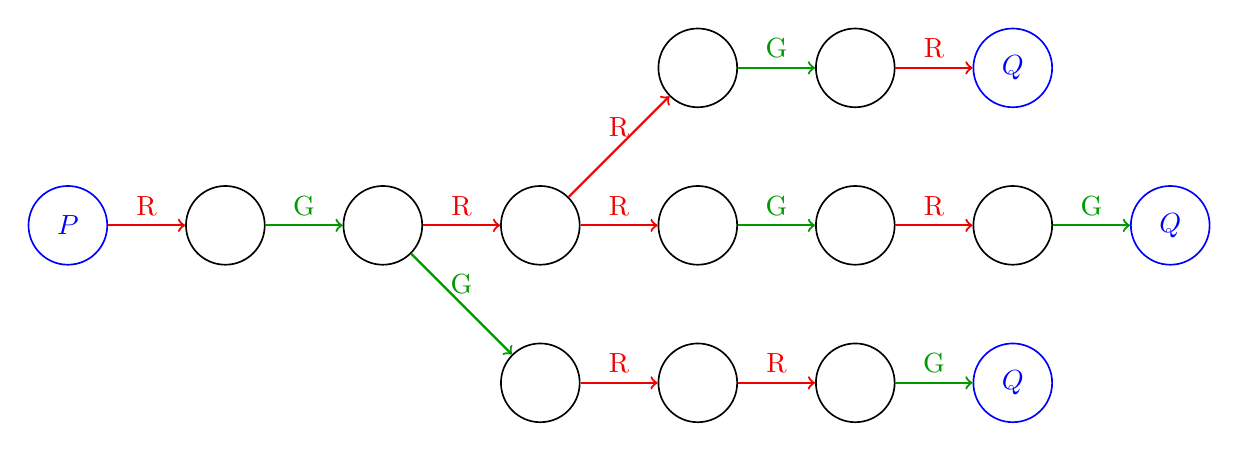
\begin{tikzpicture}[->, semithick]
\tikzset{
    prepost/.style= {circle, draw=blue, color=blue, minimum size=1.0cm},
    pstate/.style= {circle, draw=black, minimum size=1.0cm},
    prel/.style= {above, black!5!red, thick},
    pguar/.style= {above, black!40!green, thick},
}

\node[prepost] (P) at (0,0) {$P$};
\node[pstate] (s1) at (2,0) {};
\node[pstate] (s2) at (4,0) {};
\node[pstate] (s3) at (6,0) {};
\node[pstate] (s4) at (8,0) {};
\node[pstate] (s5) at (10,0) {};
\node[pstate] (s6) at (12,0) {};
\node[prepost] (s7) at (14,0) {$Q$};

\node[pstate] (s8) at (8,2) {};
\node[pstate] (s9) at (10,2) {};
\node[prepost] (s10) at (12,2) {$Q$};

\node[pstate] (s11) at (6,-2) {};
\node[pstate] (s12) at (8,-2) {};
\node[pstate] (s13) at (10,-2) {};
\node[prepost] (s14) at (12,-2) {$Q$};

\draw
(P) edge[prel] node {R} (s1)
(s1) edge[pguar] node {G} (s2)
(s2) edge[prel] node {R} (s3)
(s3) edge[prel] node {R} (s4)
(s4) edge[pguar] node {G} (s5)
(s5) edge[prel] node {R} (s6)
(s6) edge[pguar] node {G} (s7)
(s3) edge[prel] node {R} (s8)
(s8) edge[pguar] node {G} (s9)
(s9) edge[prel] node {R} (s10)
(s2) edge[pguar] node {G} (s11)
(s11) edge[prel] node {R} (s12)
(s12) edge[prel] node {R} (s13)
(s13) edge[pguar] node {G} (s14);
\end{tikzpicture}
\end{center}
\fi
\end{document}